% =============================================================================
% PART B - MODULE 14: FORUM MANAGEMENT (UC-14.01 - UC-14.17)
% In Charge: Pham Kha Vy
% =============================================================================
\subsection{Module 14: Forum Management}

\subsubsection{M14.01 -- View Forum Category List (UC-14.01)}
\begin{itemize}[leftmargin=1.5em,itemsep=2pt]
  \item \textbf{Screen Name \& Route Path:} Forum Home -- \texttt{/forum}.
  \item \textbf{Who Can Use This:} Client, Freelancer.
  \item \Needspace{6\baselineskip}\textbf{Before You Begin:} User has navigated to the community forum section.
\end{itemize}
\begin{figure}[H]\centering
  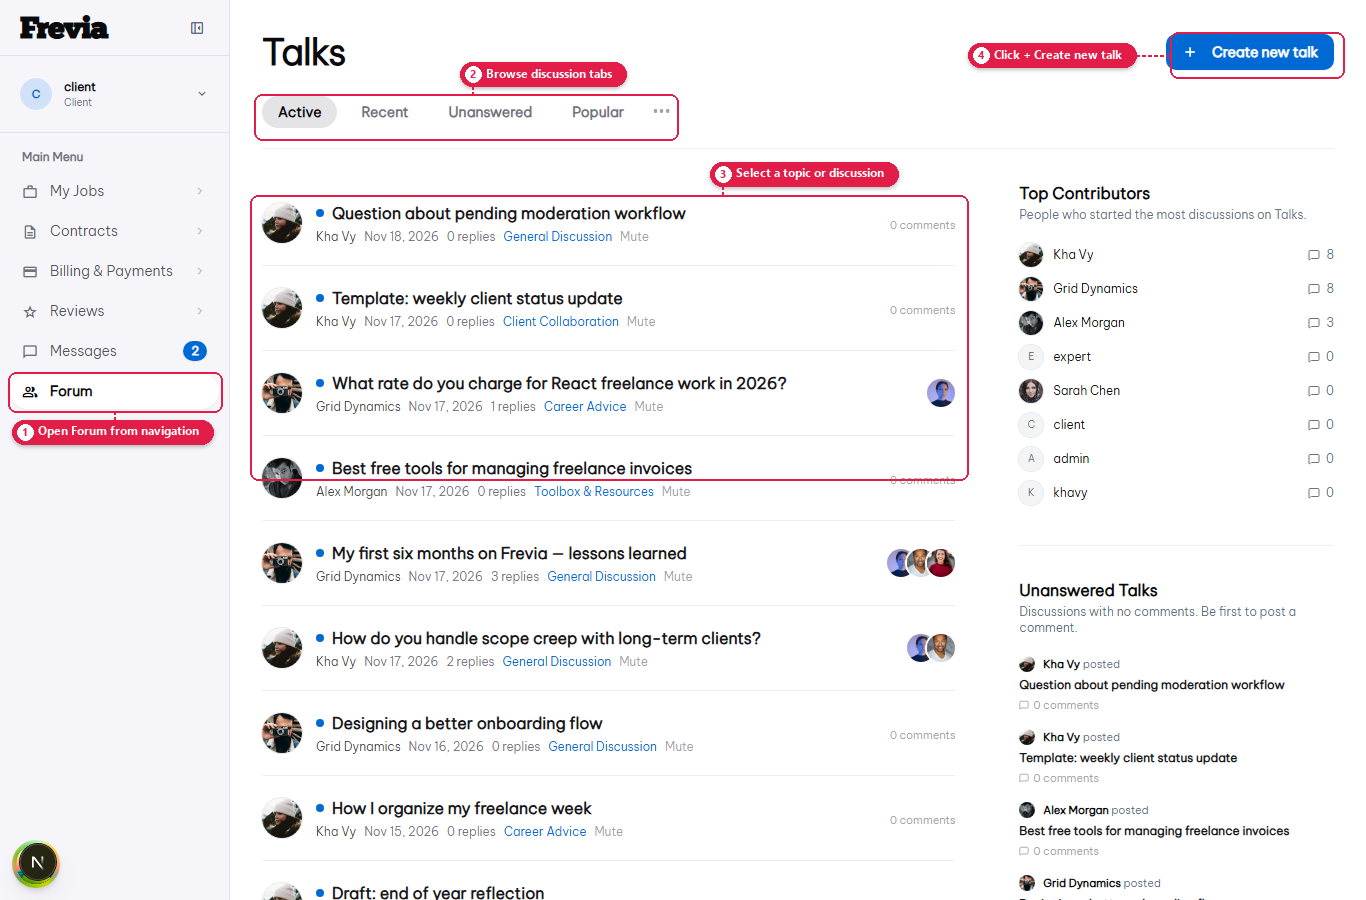
\includegraphics[width=0.90\textwidth]{images/forum/f14_01_guide.png}
  \caption{Forum home displaying discussion tabs and categories}
\end{figure}
\Needspace{6\baselineskip}\paragraph{Step-by-Step User Guide:}
\begin{enumerate}[leftmargin=1.8em,itemsep=3pt]
  \item \rbadge{1} \textbf{Open Forum Navigation:} Click \textbf{Forum} in the left sidebar to open the community hub.
  \item \rbadge{2} \textbf{Browse Tabs \& Categories:} Use the top filter tabs (Active, Recent, Unanswered, Popular) or category links to filter discussions.
  \item \rbadge{3} \textbf{Select Discussion or Category:} Click any category or discussion topic card to inspect its threads.
  \item \rbadge{4} \textbf{Create New Talk:} Click the blue \textbf{+ Create new talk} button at the top-right to start a new thread.
\end{enumerate}
\Needspace{6\baselineskip}\paragraph{After You Submit (Result \& Troubleshooting):}
\begin{itemize}[leftmargin=1.5em,itemsep=2pt]
  \item \textbf{What Happens Next:} All active forum categories are displayed with names, descriptions, and post counts.
  \item \textbf{Troubleshooting \& Common Messages:} If no categories are configured yet, an empty-state placeholder is displayed.
\end{itemize}

\subsubsection{M14.02 -- View Forum Category Detail (UC-14.02)}
\begin{itemize}[leftmargin=1.5em,itemsep=2pt]
  \item \textbf{Screen Name \& Route Path:} Category Detail -- \texttt{/forum/\{categorySlug\}}.
  \item \textbf{Who Can Use This:} Client, Freelancer.
  \item \Needspace{6\baselineskip}\textbf{Before You Begin:} At least one active forum category exists.
\end{itemize}
\begin{figure}[H]\centering
  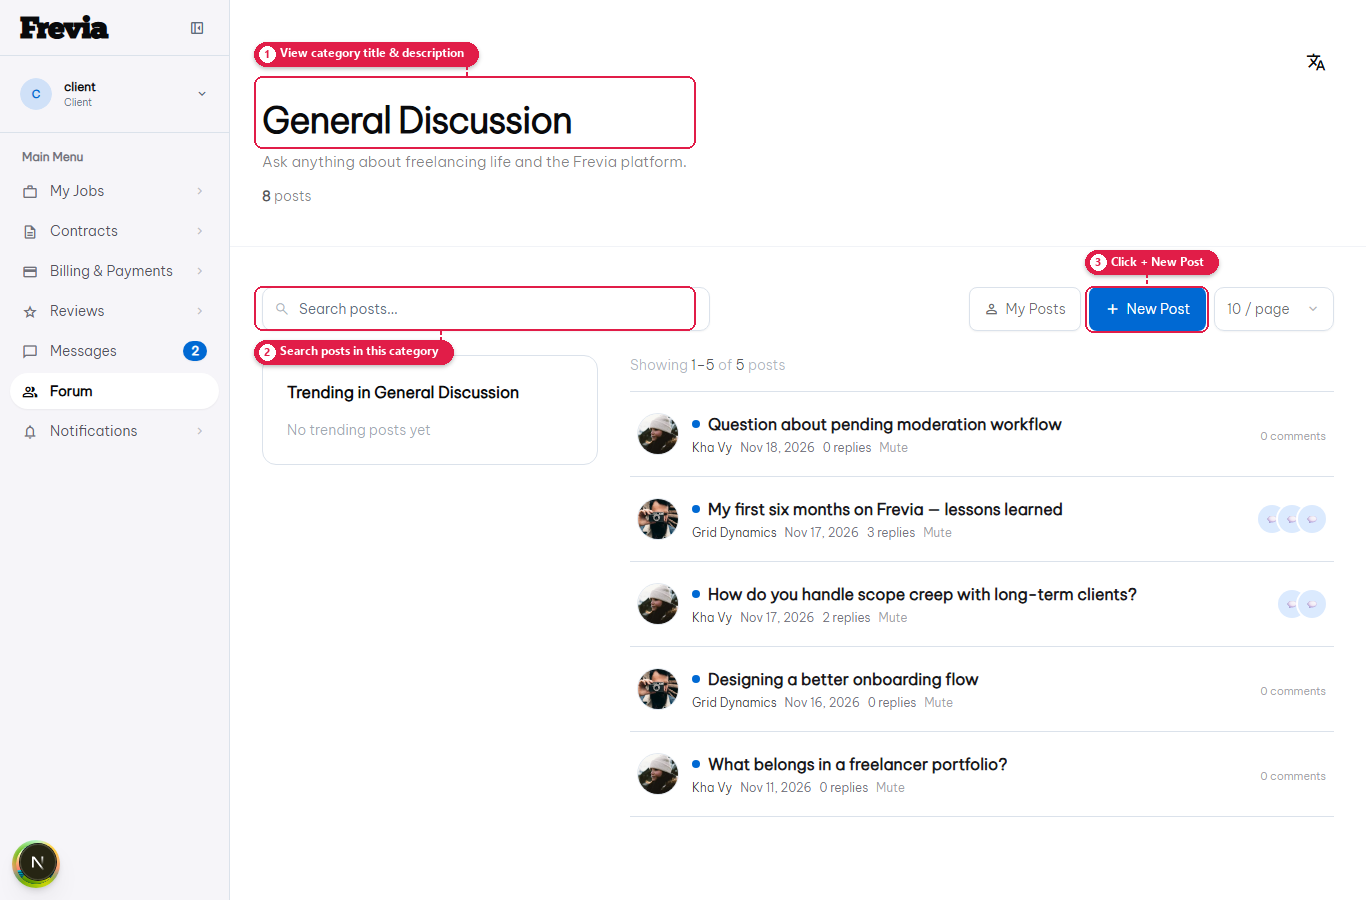
\includegraphics[width=0.90\textwidth]{images/forum/f14_02_guide.png}
  \caption{Forum category detail page with search and post creation}
\end{figure}
\Needspace{6\baselineskip}\paragraph{Step-by-Step User Guide:}
\begin{enumerate}[leftmargin=1.8em,itemsep=3pt]
  \item \rbadge{1} \textbf{View Category Header:} Inspect the selected category title and description at the top of the page.
  \item \rbadge{2} \textbf{Search \& Filter Posts:} Type keywords into the search bar to filter threads inside this category.
  \item \rbadge{3} \textbf{Create Category Post:} Click \textbf{+ New Post} to author a post pre-tagged to this category.
\end{enumerate}
\Needspace{6\baselineskip}\paragraph{After You Submit (Result \& Troubleshooting):}
\begin{itemize}[leftmargin=1.5em,itemsep=2pt]
  \item \textbf{What Happens Next:} The category header and its paginated discussion list are rendered.
  \item \textbf{Troubleshooting \& Common Messages:} If the category slug is invalid or soft-deleted, a 404 Not Found message is shown.
\end{itemize}

\subsubsection{M14.03 -- View Post List (UC-14.03)}
\begin{itemize}[leftmargin=1.5em,itemsep=2pt]
  \item \textbf{Screen Name \& Route Path:} Forum Post List -- \texttt{/forum/\{categorySlug\}}.
  \item \textbf{Who Can Use This:} Client, Freelancer.
  \item \Needspace{6\baselineskip}\textbf{Before You Begin:} User is viewing a forum category or global feed.
\end{itemize}
\begin{figure}[H]\centering
  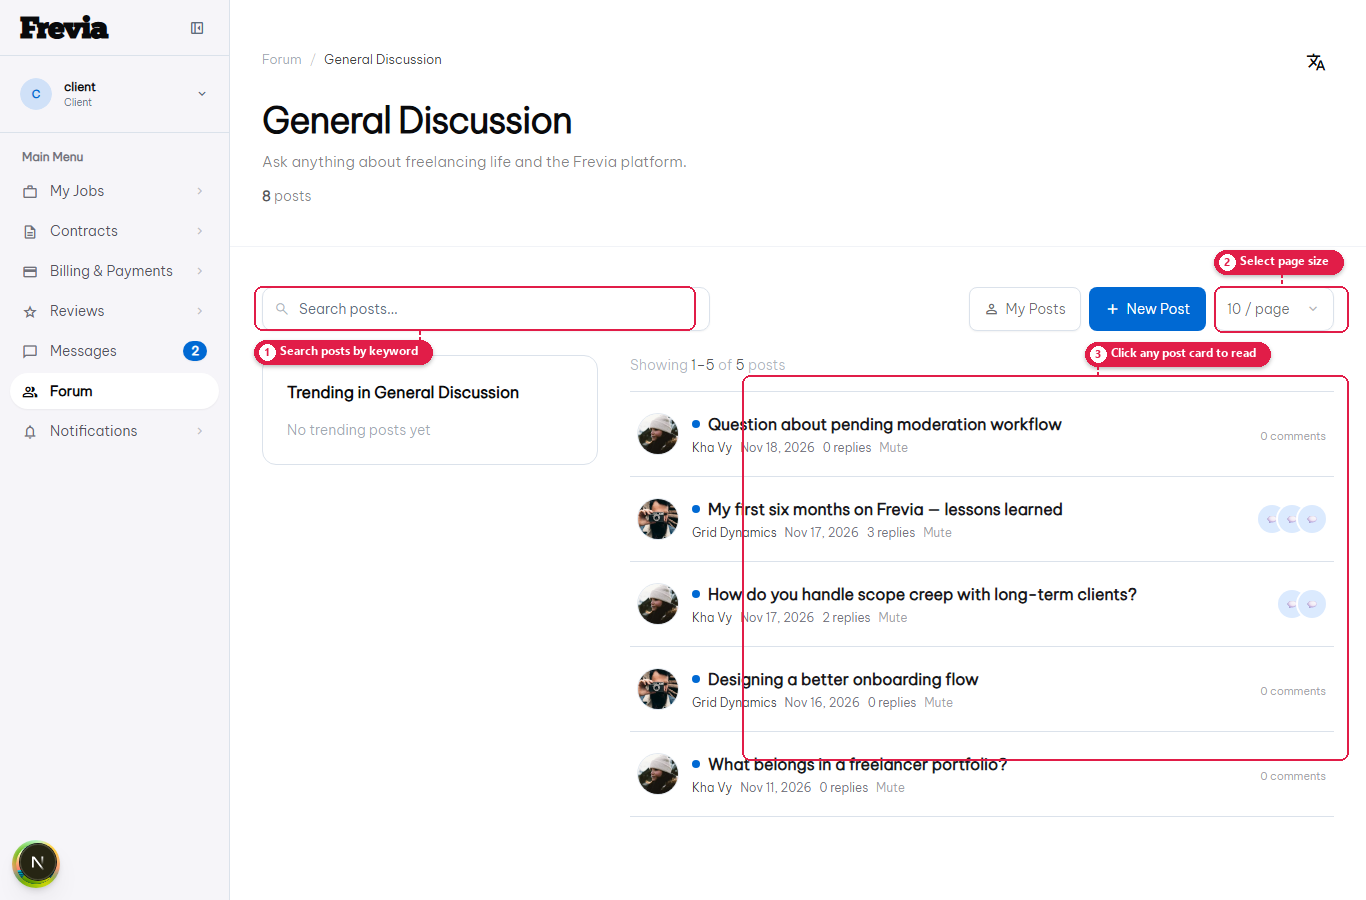
\includegraphics[width=0.90\textwidth]{images/forum/f14_03_guide.png}
  \caption{Paginated list of approved forum posts}
\end{figure}
\Needspace{6\baselineskip}\paragraph{Step-by-Step User Guide:}
\begin{enumerate}[leftmargin=1.8em,itemsep=3pt]
  \item \rbadge{1} \textbf{Search by Keyword:} Enter a topic keyword in the search bar to filter approved posts.
  \item \rbadge{2} \textbf{Adjust Pagination:} Use the page size selector (e.g., 10 / page) and page controls to navigate results.
  \item \rbadge{3} \textbf{Open Post Detail:} Click any post title card to open the full discussion thread.
\end{enumerate}
\Needspace{6\baselineskip}\paragraph{After You Submit (Result \& Troubleshooting):}
\begin{itemize}[leftmargin=1.5em,itemsep=2pt]
  \item \textbf{What Happens Next:} Approved posts are listed chronologically with author, date, and comment count.
  \item \textbf{Troubleshooting \& Common Messages:} If no posts match your search query, an empty search state is displayed.
\end{itemize}

\subsubsection{M14.04 -- View Post Detail (UC-14.04)}
\begin{itemize}[leftmargin=1.5em,itemsep=2pt]
  \item \textbf{Screen Name \& Route Path:} Post Detail -- \texttt{/forum/\{categorySlug\}/\{postSlug\}}.
  \item \textbf{Who Can Use This:} Client, Freelancer.
  \item \Needspace{6\baselineskip}\textbf{Before You Begin:} Target post is approved and publicly accessible.
\end{itemize}
\begin{figure}[H]\centering
  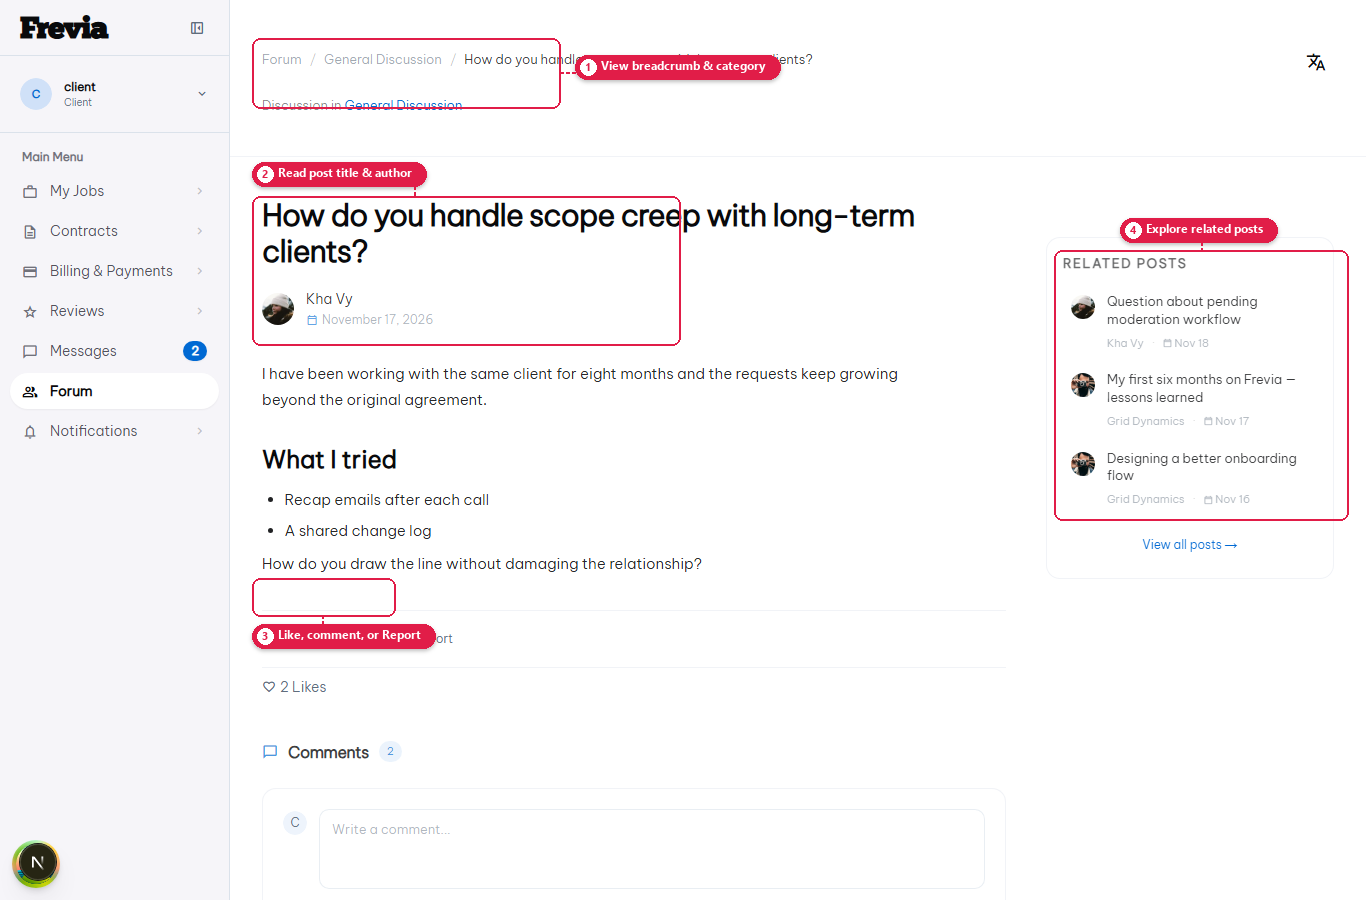
\includegraphics[width=0.90\textwidth]{images/forum/f14_04_guide.png}
  \caption{Forum post detail view with engagement bar and related posts}
\end{figure}
\Needspace{6\baselineskip}\paragraph{Step-by-Step User Guide:}
\begin{enumerate}[leftmargin=1.8em,itemsep=3pt]
  \item \rbadge{1} \textbf{Check Category Breadcrumb:} Use the top breadcrumb to see the parent category or navigate back.
  \item \rbadge{2} \textbf{Read Post Content:} Review the full formatted body, author profile, and publication timestamp.
  \item \rbadge{3} \textbf{Engage with Post:} Click the Heart icon to like, the Comment icon to jump to replies, or Report to flag violations.
  \item \rbadge{4} \textbf{Explore Related Posts:} Click any suggested thread in the right-hand Related Posts panel.
\end{enumerate}
\Needspace{6\baselineskip}\paragraph{After You Submit (Result \& Troubleshooting):}
\begin{itemize}[leftmargin=1.5em,itemsep=2pt]
  \item \textbf{What Happens Next:} Full post details, engagement counts, and comment thread load cleanly.
  \item \textbf{Troubleshooting \& Common Messages:} If the post was removed or rejected, an unavailable notice is shown.
\end{itemize}

\subsubsection{M14.05 -- Create Post (UC-14.05)}
\begin{itemize}[leftmargin=1.5em,itemsep=2pt]
  \item \textbf{Screen Name \& Route Path:} Create Post Modal -- \texttt{/forum/\{categorySlug\}}.
  \item \textbf{Who Can Use This:} Client, Freelancer.
  \item \Needspace{6\baselineskip}\textbf{Before You Begin:} User is signed in to an active account.
\end{itemize}
\begin{figure}[H]\centering
  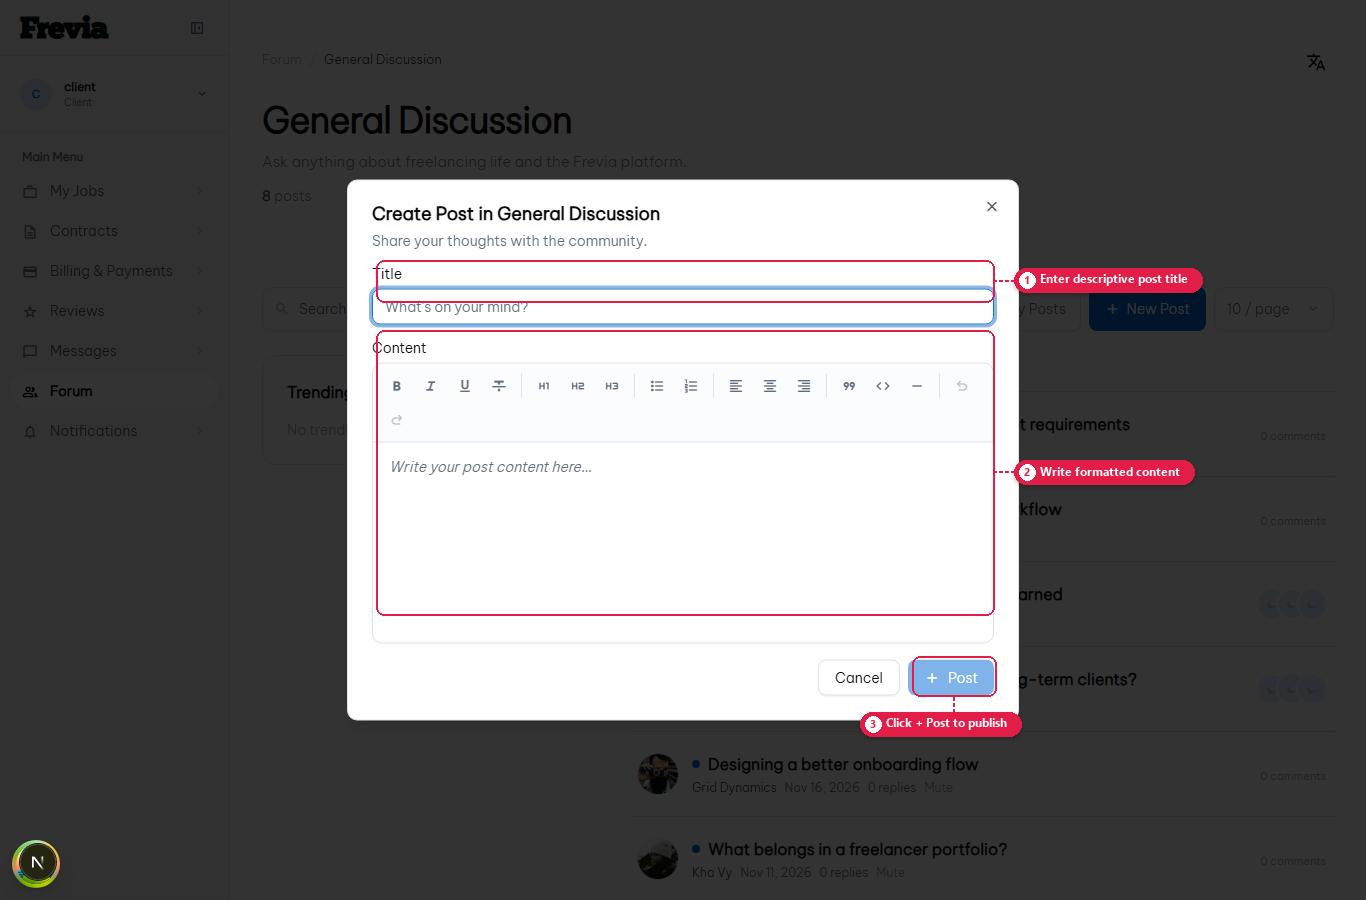
\includegraphics[width=0.90\textwidth]{images/forum/f14_05_guide.png}
  \caption{Create Post dialog with rich-text editor}
\end{figure}
\Needspace{6\baselineskip}\paragraph{Step-by-Step User Guide:}
\begin{enumerate}[leftmargin=1.8em,itemsep=3pt]
  \item \rbadge{1} \textbf{Enter Post Title:} Type a clear, descriptive title into the \textit{Title} field.
  \item \rbadge{2} \textbf{Write Formatted Content:} Compose your discussion in the rich-text editor using headings, lists, or code blocks.
  \item \rbadge{3} \textbf{Publish Post:} Click \textbf{+ Post} to run automated AI moderation and submit the thread.
\end{enumerate}
\Needspace{6\baselineskip}\paragraph{After You Submit (Result \& Troubleshooting):}
\begin{itemize}[leftmargin=1.5em,itemsep=2pt]
  \item \textbf{What Happens Next:} Posts with low AI risk scores publish immediately; borderline posts enter Pending review.
  \item \textbf{Troubleshooting \& Common Messages:} Empty required fields trigger validation warnings; severely toxic content is blocked.
\end{itemize}

\subsubsection{M14.06 -- Update Post (UC-14.06)}
\begin{itemize}[leftmargin=1.5em,itemsep=2pt]
  \item \textbf{Screen Name \& Route Path:} Edit Post Modal -- \texttt{/forum/\{categorySlug\}/\{postSlug\}}.
  \item \textbf{Who Can Use This:} Client, Freelancer (Author only).
  \item \Needspace{6\baselineskip}\textbf{Before You Begin:} User is the original author of the post.
\end{itemize}
\begin{figure}[H]\centering
  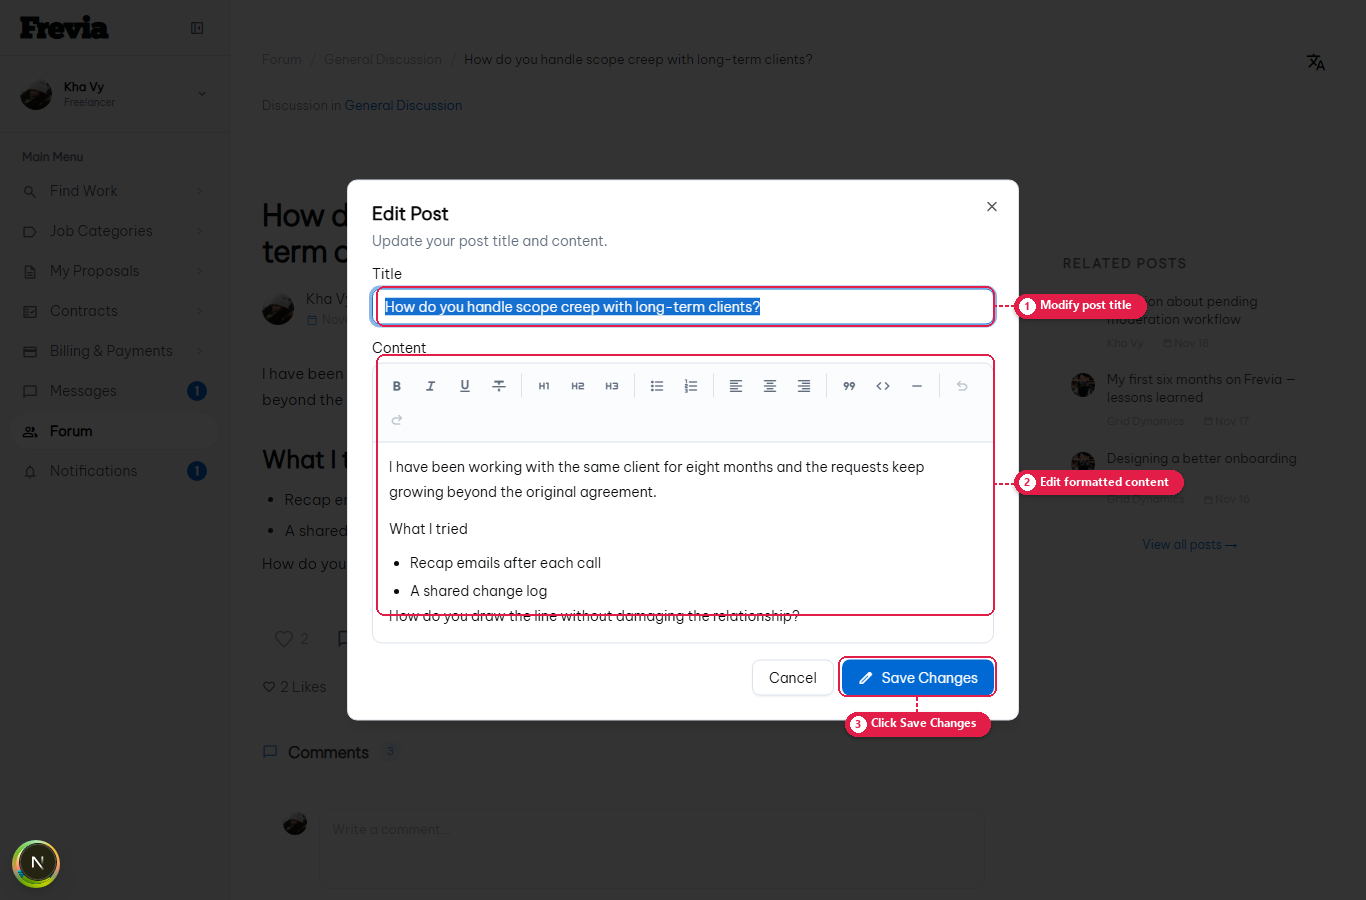
\includegraphics[width=0.90\textwidth]{images/forum/f14_06_guide.png}
  \caption{Update Post modal for editing title or body}
\end{figure}
\Needspace{6\baselineskip}\paragraph{Step-by-Step User Guide:}
\begin{enumerate}[leftmargin=1.8em,itemsep=3pt]
  \item \rbadge{1} \textbf{Open Edit Dialog:} Open your own post and click the \textbf{Edit} action button.
  \item \rbadge{2} \textbf{Modify Title or Content:} Update the post title, category, or rich-text content.
  \item \rbadge{3} \textbf{Save Changes:} Click \textbf{Save} to persist the updated post.
\end{enumerate}
\Needspace{6\baselineskip}\paragraph{After You Submit (Result \& Troubleshooting):}
\begin{itemize}[leftmargin=1.5em,itemsep=2pt]
  \item \textbf{What Happens Next:} Your post updates immediately with the revised content.
  \item \textbf{Troubleshooting \& Common Messages:} Non-authors do not see the Edit action; invalid inputs are rejected.
\end{itemize}

\subsubsection{M14.07 -- Delete Post (UC-14.07)}
\begin{itemize}[leftmargin=1.5em,itemsep=2pt]
  \item \textbf{Screen Name \& Route Path:} Delete Post Dialog -- \texttt{/forum/\{categorySlug\}/\{postSlug\}}.
  \item \textbf{Who Can Use This:} Client, Freelancer (Author only).
  \item \Needspace{6\baselineskip}\textbf{Before You Begin:} User is the original author of the post.
\end{itemize}
\begin{figure}[H]\centering
  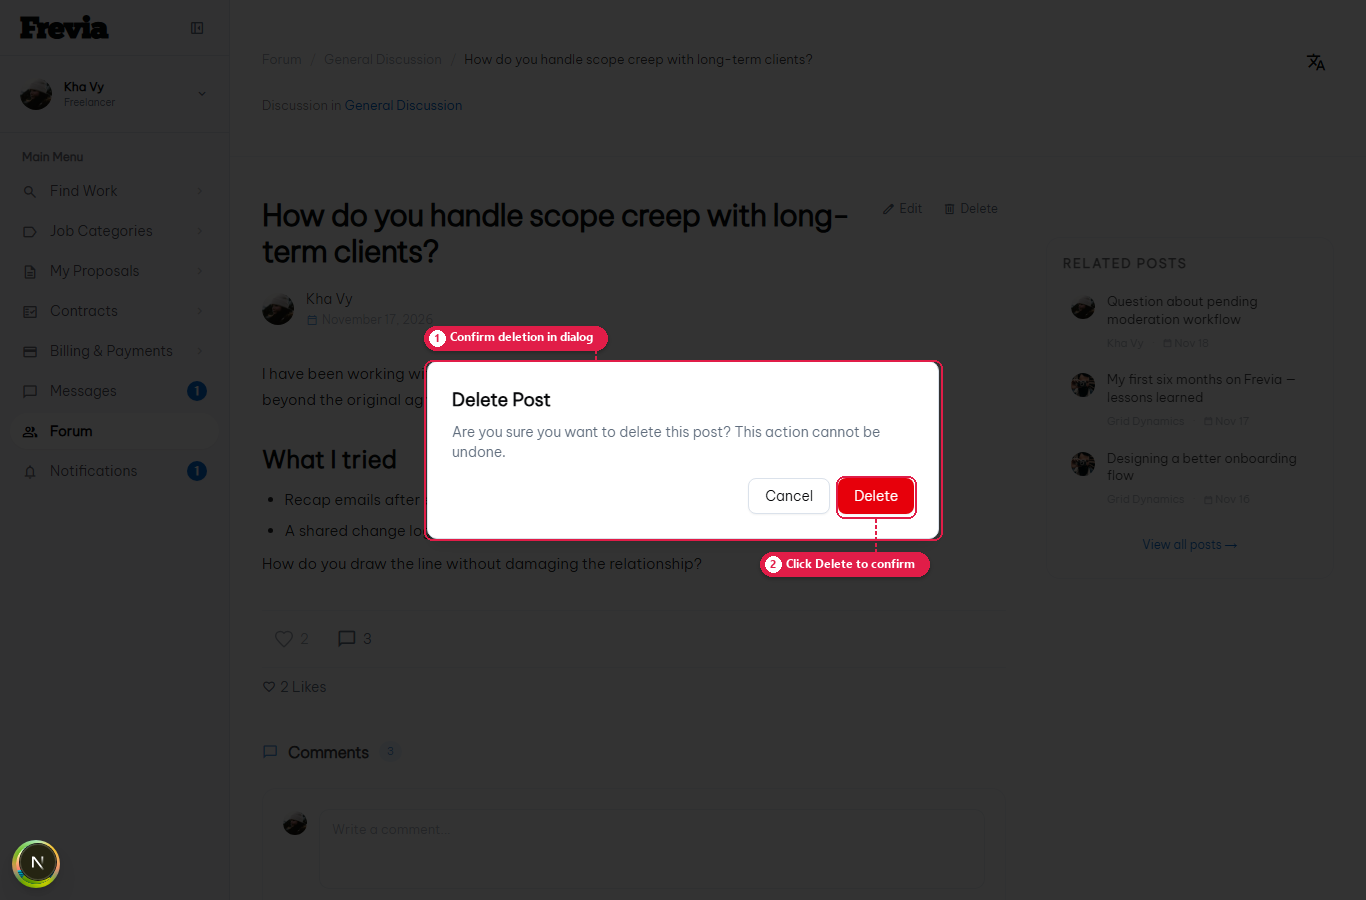
\includegraphics[width=0.90\textwidth]{images/forum/f14_07_guide.png}
  \caption{Soft-delete confirmation dialog for forum post}
\end{figure}
\Needspace{6\baselineskip}\paragraph{Step-by-Step User Guide:}
\begin{enumerate}[leftmargin=1.8em,itemsep=3pt]
  \item \rbadge{1} \textbf{Trigger Delete:} Open your own post and click the \textbf{Delete} button.
  \item \rbadge{2} \textbf{Review Confirmation:} Read the soft-deletion warning inside the confirmation modal.
  \item \rbadge{3} \textbf{Confirm Deletion:} Click \textbf{Confirm Delete} to move the post to Admin Forum Trash.
\end{enumerate}
\Needspace{6\baselineskip}\paragraph{After You Submit (Result \& Troubleshooting):}
\begin{itemize}[leftmargin=1.5em,itemsep=2pt]
  \item \textbf{What Happens Next:} The post is soft-deleted and removed from public forum listings.
  \item \textbf{Troubleshooting \& Common Messages:} Unauthorized users cannot delete posts authored by others.
\end{itemize}

\subsubsection{M14.08 -- Like Post (UC-14.08)}
\begin{itemize}[leftmargin=1.5em,itemsep=2pt]
  \item \textbf{Screen Name \& Route Path:} Post Detail -- \texttt{/forum/\{categorySlug\}/\{postSlug\}}.
  \item \textbf{Who Can Use This:} Client, Freelancer.
  \item \Needspace{6\baselineskip}\textbf{Before You Begin:} User is signed in and has not yet liked the post.
\end{itemize}
\begin{figure}[H]\centering
  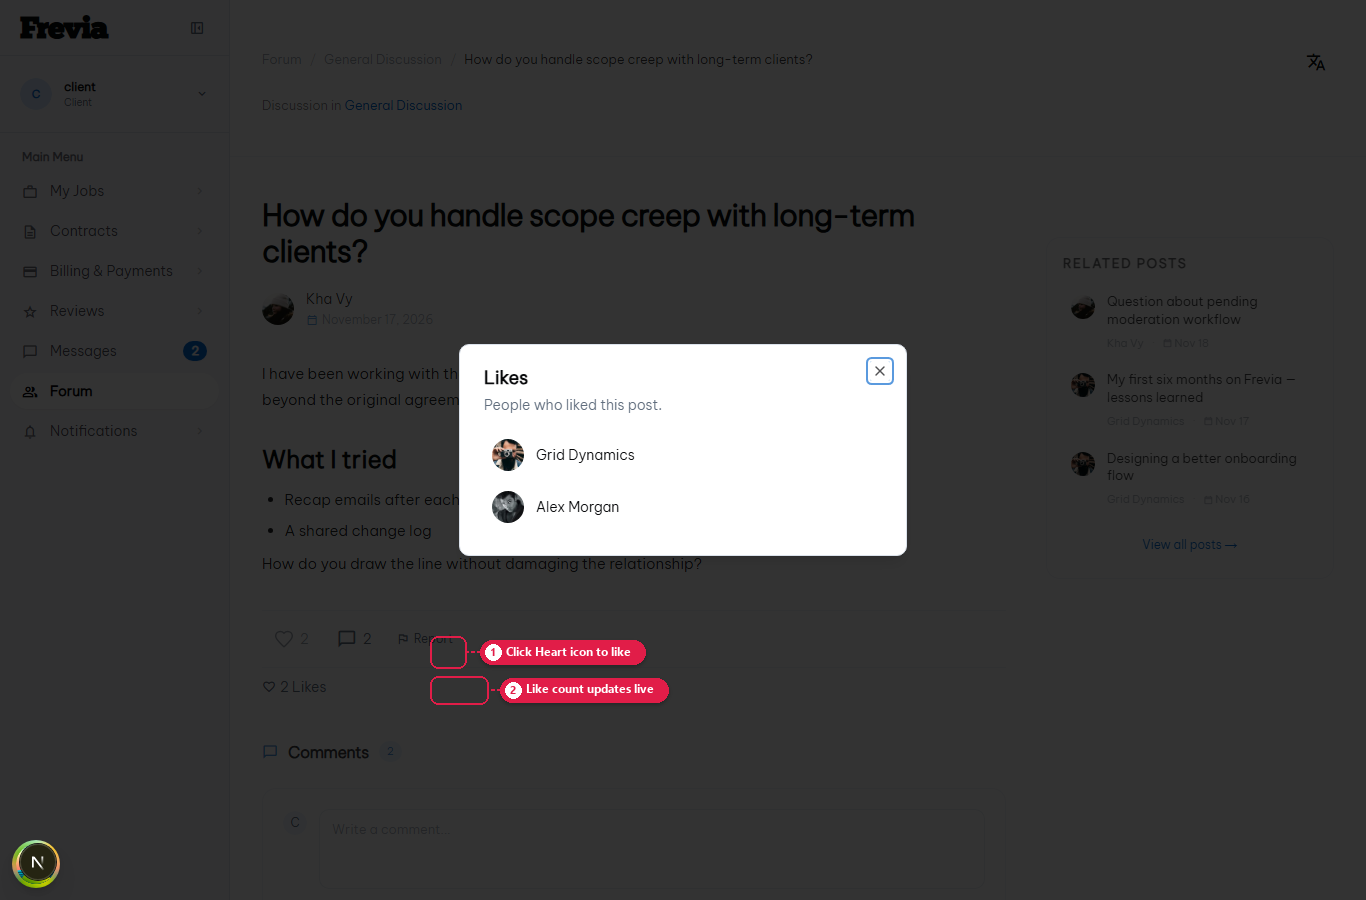
\includegraphics[width=0.90\textwidth]{images/forum/f14_08_guide.png}
  \caption{Liking a forum post}
\end{figure}
\Needspace{6\baselineskip}\paragraph{Step-by-Step User Guide:}
\begin{enumerate}[leftmargin=1.8em,itemsep=3pt]
  \item \rbadge{1} \textbf{Click Heart Icon:} Click the outline Heart button below the post body.
  \item \rbadge{2} \textbf{Verify Counter Update:} Observe the Heart icon turn active and the like counter increment by 1.
\end{enumerate}
\Needspace{6\baselineskip}\paragraph{After You Submit (Result \& Troubleshooting):}
\begin{itemize}[leftmargin=1.5em,itemsep=2pt]
  \item \textbf{What Happens Next:} Your reaction is saved and reflected in real time.
  \item \textbf{Troubleshooting \& Common Messages:} Unauthenticated visitors are prompted to sign in before liking.
\end{itemize}

\subsubsection{M14.09 -- Unlike Post (UC-14.09)}
\begin{itemize}[leftmargin=1.5em,itemsep=2pt]
  \item \textbf{Screen Name \& Route Path:} Post Detail -- \texttt{/forum/\{categorySlug\}/\{postSlug\}}.
  \item \textbf{Who Can Use This:} Client, Freelancer.
  \item \Needspace{6\baselineskip}\textbf{Before You Begin:} User has previously liked the post.
\end{itemize}
\begin{figure}[H]\centering
  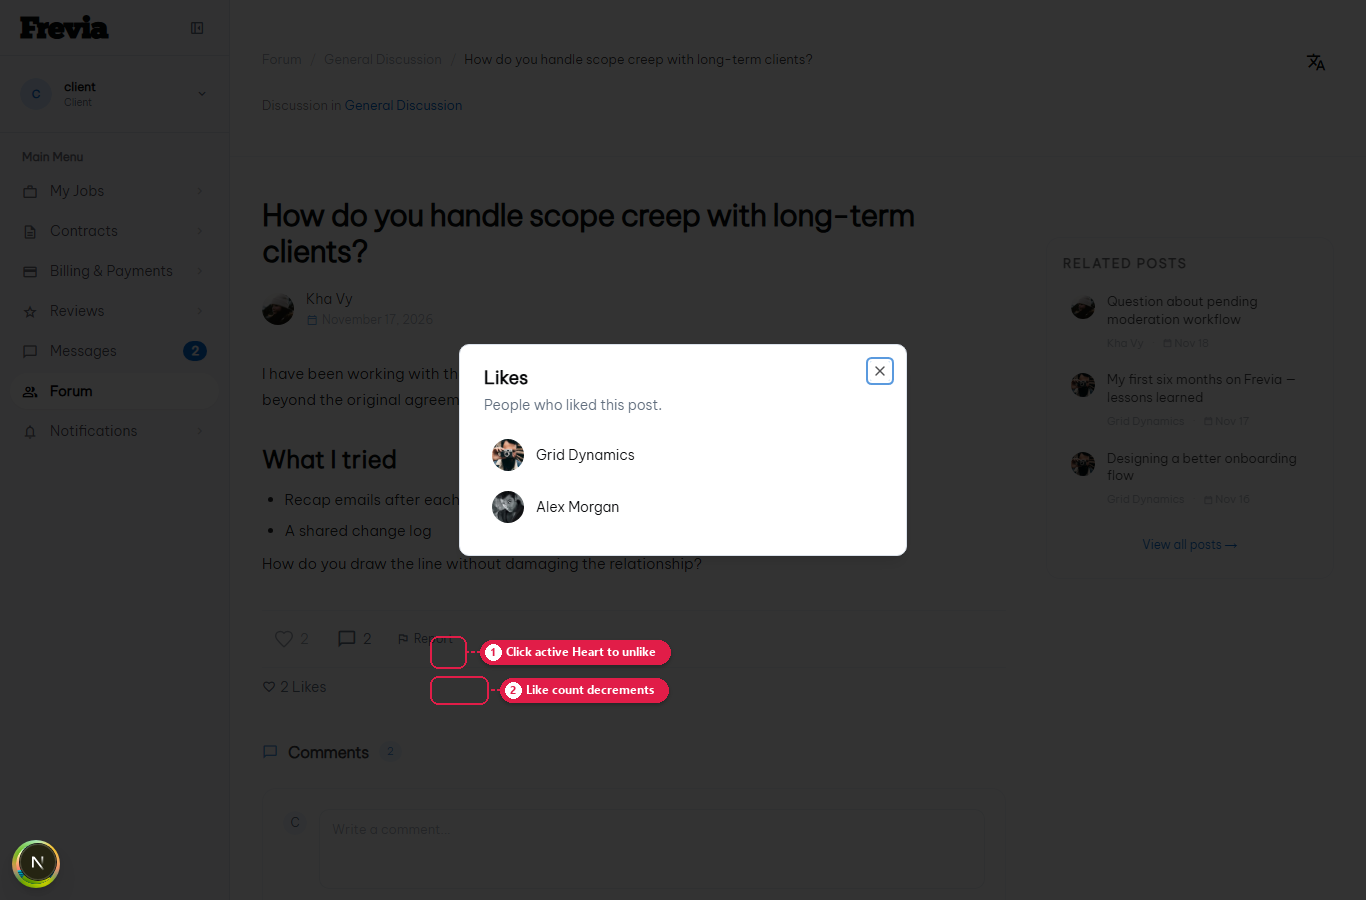
\includegraphics[width=0.90\textwidth]{images/forum/f14_09_guide.png}
  \caption{Removing a like from a forum post}
\end{figure}
\Needspace{6\baselineskip}\paragraph{Step-by-Step User Guide:}
\begin{enumerate}[leftmargin=1.8em,itemsep=3pt]
  \item \rbadge{1} \textbf{Click Active Heart Icon:} Click the highlighted Heart icon below the post body.
  \item \rbadge{2} \textbf{Verify Counter Decrement:} Observe the Heart return to outline state and the counter decrement by 1.
\end{enumerate}
\Needspace{6\baselineskip}\paragraph{After You Submit (Result \& Troubleshooting):}
\begin{itemize}[leftmargin=1.5em,itemsep=2pt]
  \item \textbf{What Happens Next:} Your like record is removed immediately.
  \item \textbf{Troubleshooting \& Common Messages:} If the post was deleted concurrently, a not-found toast is displayed.
\end{itemize}

\subsubsection{M14.10 -- View Post Likes (UC-14.10)}
\begin{itemize}[leftmargin=1.5em,itemsep=2pt]
  \item \textbf{Screen Name \& Route Path:} Post Likes Modal -- \texttt{/forum/\{categorySlug\}/\{postSlug\}}.
  \item \textbf{Who Can Use This:} Client, Freelancer.
  \item \Needspace{6\baselineskip}\textbf{Before You Begin:} Post has at least one like.
\end{itemize}
\begin{figure}[H]\centering
  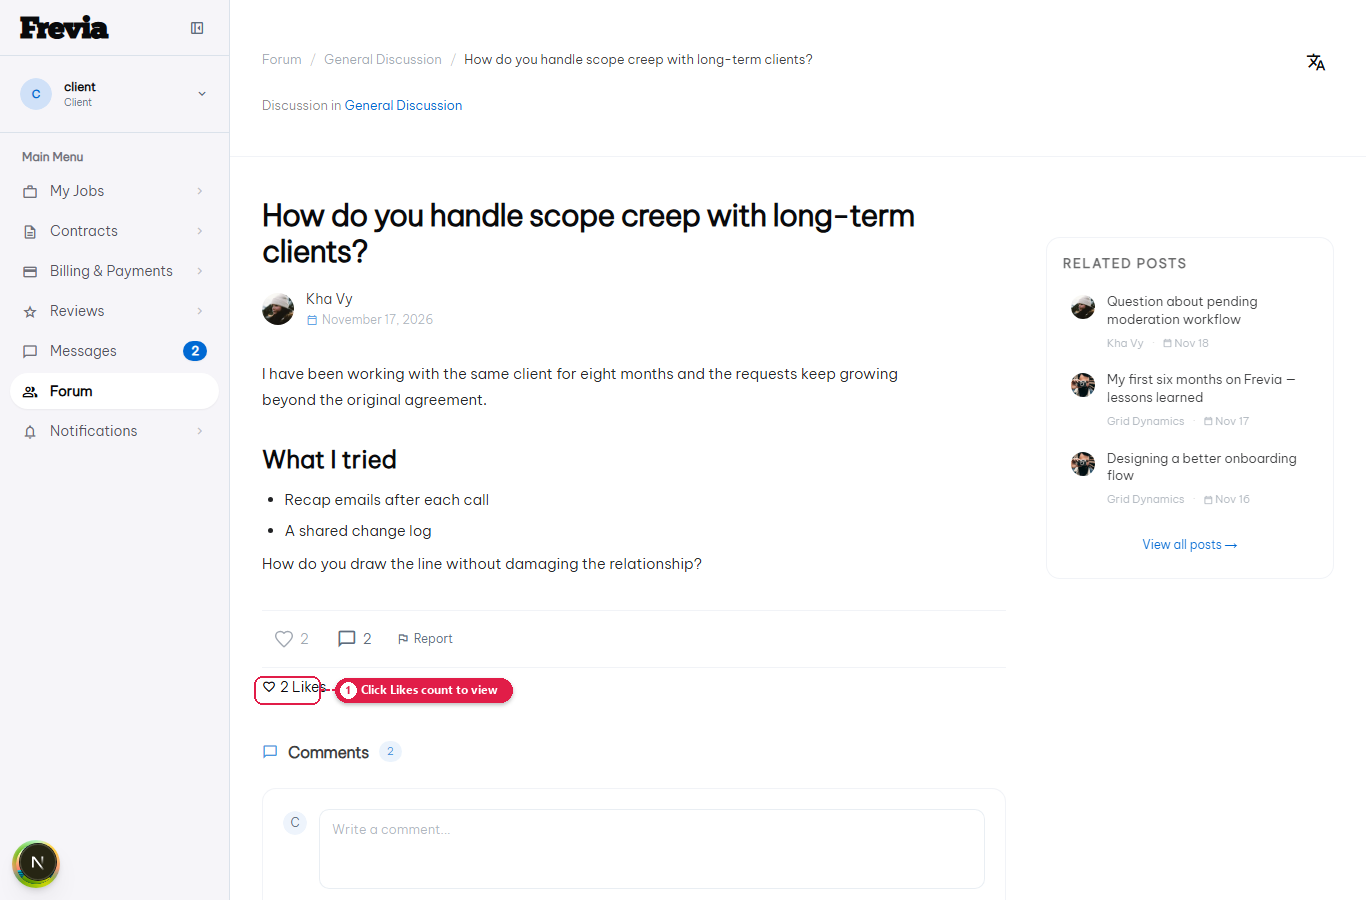
\includegraphics[width=0.90\textwidth]{images/forum/f14_10_guide.png}
  \caption{Modal showing users who liked the post}
\end{figure}
\Needspace{6\baselineskip}\paragraph{Step-by-Step User Guide:}
\begin{enumerate}[leftmargin=1.8em,itemsep=3pt]
  \item \rbadge{1} \textbf{Click Likes Summary:} Click the \textit{Likes} count link beneath the post engagement bar.
  \item \rbadge{2} \textbf{Browse Liked Users:} Inspect the list of community members who reacted to the post.
\end{enumerate}
\Needspace{6\baselineskip}\paragraph{After You Submit (Result \& Troubleshooting):}
\begin{itemize}[leftmargin=1.5em,itemsep=2pt]
  \item \textbf{What Happens Next:} A modal displays avatars and names of all users who liked the post.
  \item \textbf{Troubleshooting \& Common Messages:} If no likes exist, an empty list message is shown.
\end{itemize}

\subsubsection{M14.11 -- View Post Comments (UC-14.11)}
\begin{itemize}[leftmargin=1.5em,itemsep=2pt]
  \item \textbf{Screen Name \& Route Path:} Comments Section -- \texttt{/forum/\{categorySlug\}/\{postSlug\}}.
  \item \textbf{Who Can Use This:} Client, Freelancer.
  \item \Needspace{6\baselineskip}\textbf{Before You Begin:} Post is approved and visible.
\end{itemize}
\begin{figure}[H]\centering
  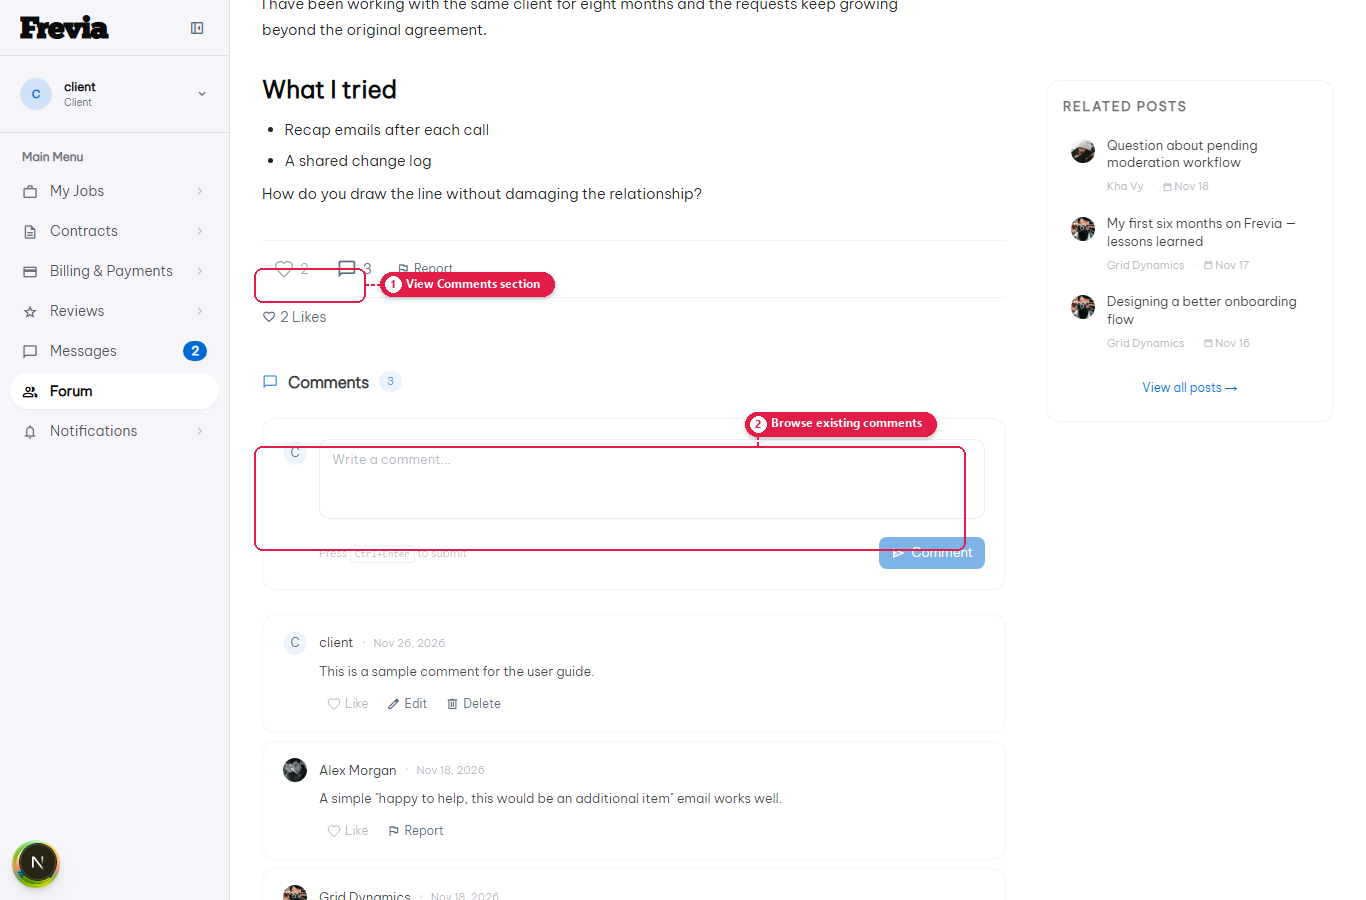
\includegraphics[width=0.90\textwidth]{images/forum/f14_11_guide.png}
  \caption{Viewing post comments thread}
\end{figure}
\Needspace{6\baselineskip}\paragraph{Step-by-Step User Guide:}
\begin{enumerate}[leftmargin=1.8em,itemsep=3pt]
  \item \rbadge{1} \textbf{Scroll to Comments:} Navigate to the \textit{Comments} heading below the post.
  \item \rbadge{2} \textbf{Read Replies:} Review nested comments, author names, and relative timestamps.
\end{enumerate}
\Needspace{6\baselineskip}\paragraph{After You Submit (Result \& Troubleshooting):}
\begin{itemize}[leftmargin=1.5em,itemsep=2pt]
  \item \textbf{What Happens Next:} All active comments for the post are displayed chronologically.
  \item \textbf{Troubleshooting \& Common Messages:} Deleted comments are hidden from the public comment thread.
\end{itemize}

\subsubsection{M14.12 -- Create Comment (UC-14.12)}
\begin{itemize}[leftmargin=1.5em,itemsep=2pt]
  \item \textbf{Screen Name \& Route Path:} Comment Composer -- \texttt{/forum/\{categorySlug\}/\{postSlug\}}.
  \item \textbf{Who Can Use This:} Client, Freelancer.
  \item \Needspace{6\baselineskip}\textbf{Before You Begin:} User is signed in on an active post.
\end{itemize}
\begin{figure}[H]\centering
  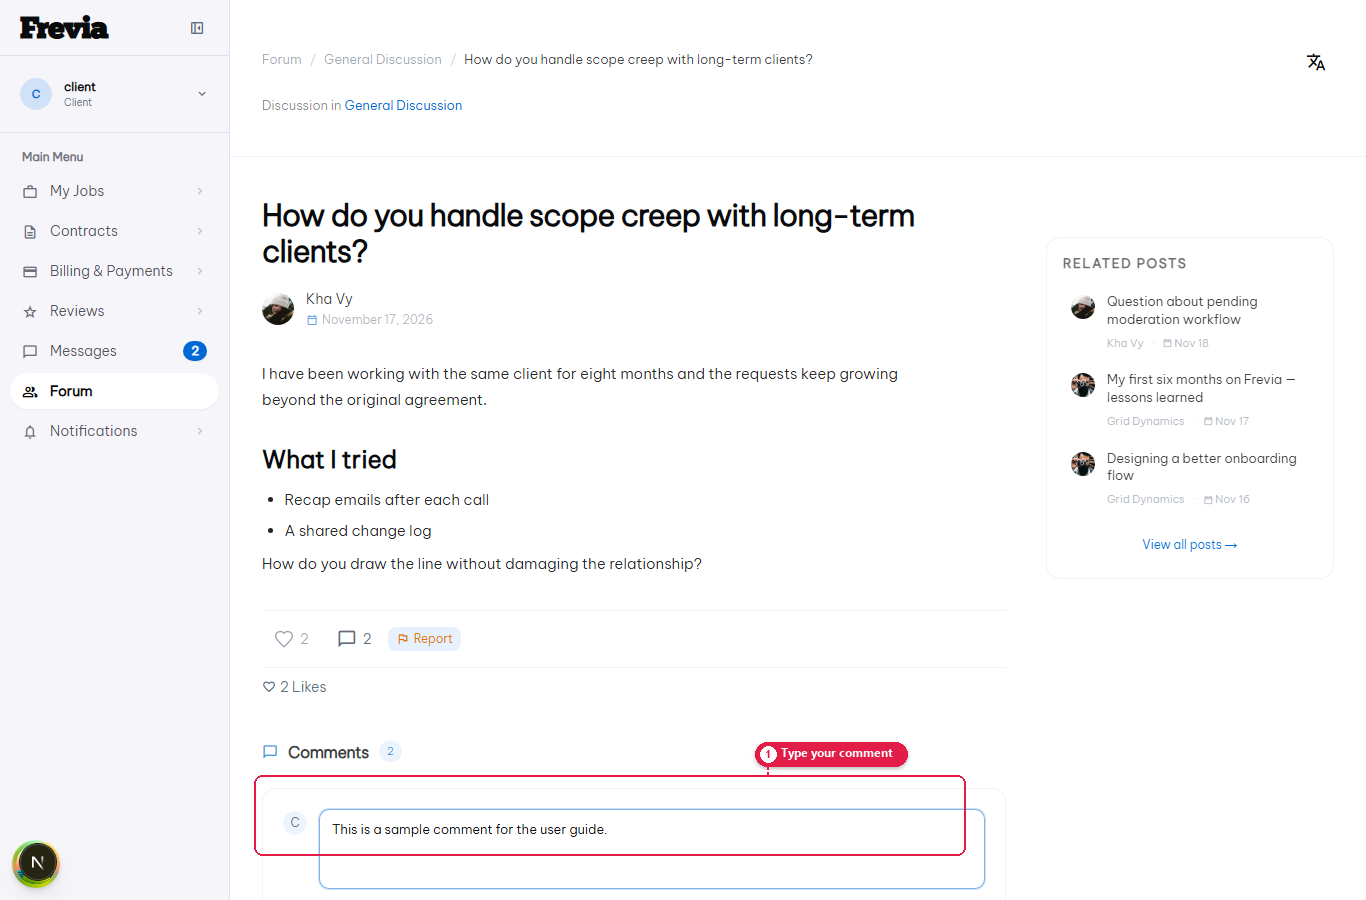
\includegraphics[width=0.90\textwidth]{images/forum/f14_12_guide.png}
  \caption{Adding a new comment to a forum post}
\end{figure}
\Needspace{6\baselineskip}\paragraph{Step-by-Step User Guide:}
\begin{enumerate}[leftmargin=1.8em,itemsep=3pt]
  \item \rbadge{1} \textbf{Type Comment:} Click into the \textit{Write a comment...} input box and enter your reply.
  \item \rbadge{2} \textbf{Submit Reply:} Click \textbf{Post Comment} to publish your response.
\end{enumerate}
\Needspace{6\baselineskip}\paragraph{After You Submit (Result \& Troubleshooting):}
\begin{itemize}[leftmargin=1.5em,itemsep=2pt]
  \item \textbf{What Happens Next:} Your comment appears immediately in the thread and increments the reply count.
  \item \textbf{Troubleshooting \& Common Messages:} Blank comments cannot be submitted.
\end{itemize}

\subsubsection{M14.13 -- Update Comment (UC-14.13)}
\begin{itemize}[leftmargin=1.5em,itemsep=2pt]
  \item \textbf{Screen Name \& Route Path:} Edit Comment -- \texttt{/forum/\{categorySlug\}/\{postSlug\}}.
  \item \textbf{Who Can Use This:} Client, Freelancer (Owner only).
  \item \Needspace{6\baselineskip}\textbf{Before You Begin:} User is the author of the target comment.
\end{itemize}
\begin{figure}[H]\centering
  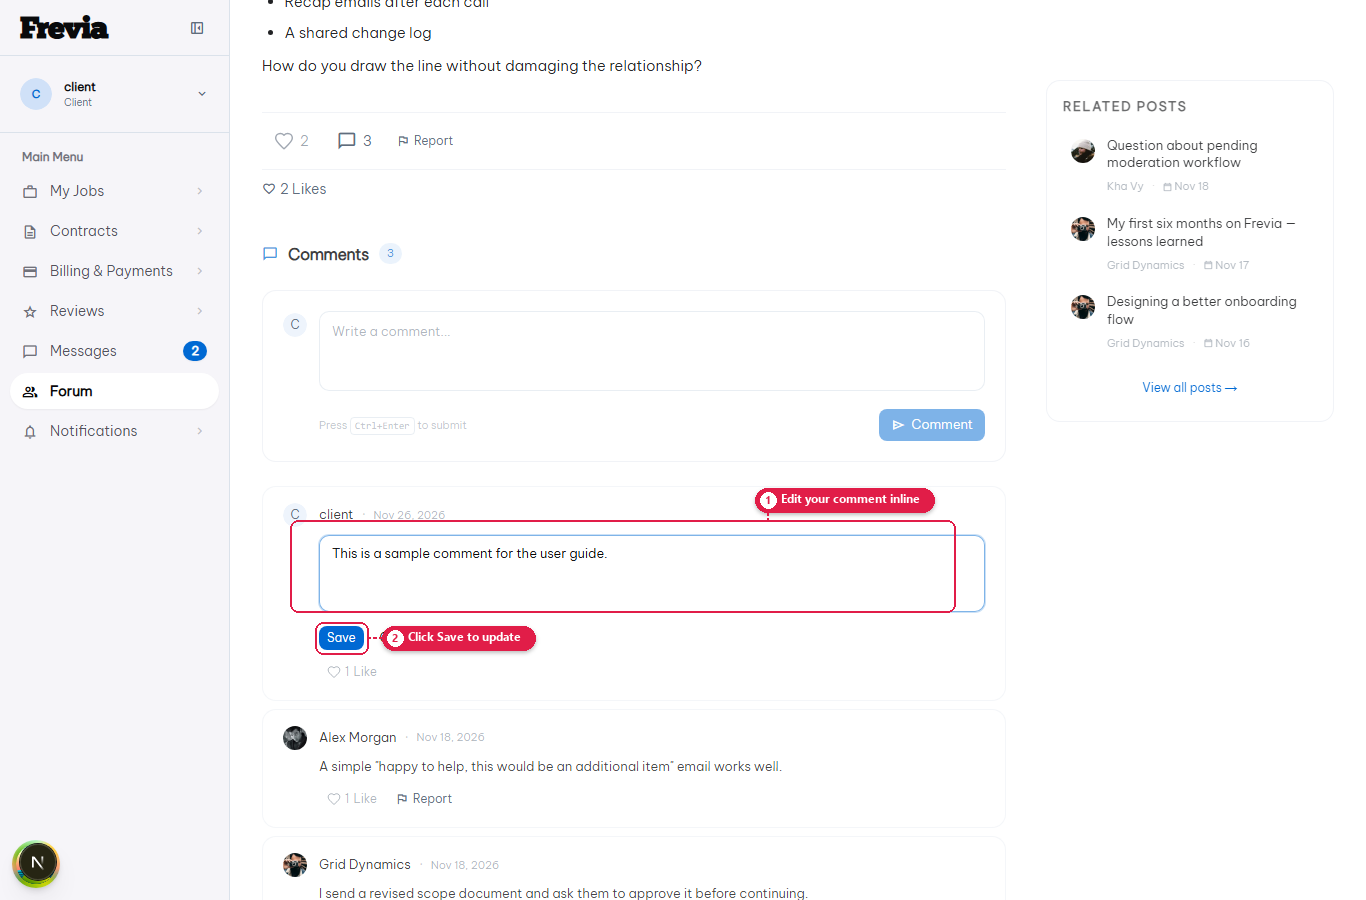
\includegraphics[width=0.90\textwidth]{images/forum/f14_13_guide.png}
  \caption{Editing an existing comment}
\end{figure}
\Needspace{6\baselineskip}\paragraph{Step-by-Step User Guide:}
\begin{enumerate}[leftmargin=1.8em,itemsep=3pt]
  \item \rbadge{1} \textbf{Open Inline Editor:} Click \textbf{Edit} on your own comment card.
  \item \rbadge{2} \textbf{Save Updated Text:} Modify your comment text and click \textbf{Save}.
\end{enumerate}
\Needspace{6\baselineskip}\paragraph{After You Submit (Result \& Troubleshooting):}
\begin{itemize}[leftmargin=1.5em,itemsep=2pt]
  \item \textbf{What Happens Next:} The comment updates in place with the revised text.
  \item \textbf{Troubleshooting \& Common Messages:} Only the comment owner can edit the comment.
\end{itemize}

\subsubsection{M14.14 -- Delete Comment (UC-14.14)}
\begin{itemize}[leftmargin=1.5em,itemsep=2pt]
  \item \textbf{Screen Name \& Route Path:} Delete Comment -- \texttt{/forum/\{categorySlug\}/\{postSlug\}}.
  \item \textbf{Who Can Use This:} Client, Freelancer (Owner only).
  \item \Needspace{6\baselineskip}\textbf{Before You Begin:} User is the author of the target comment.
\end{itemize}
\begin{figure}[H]\centering
  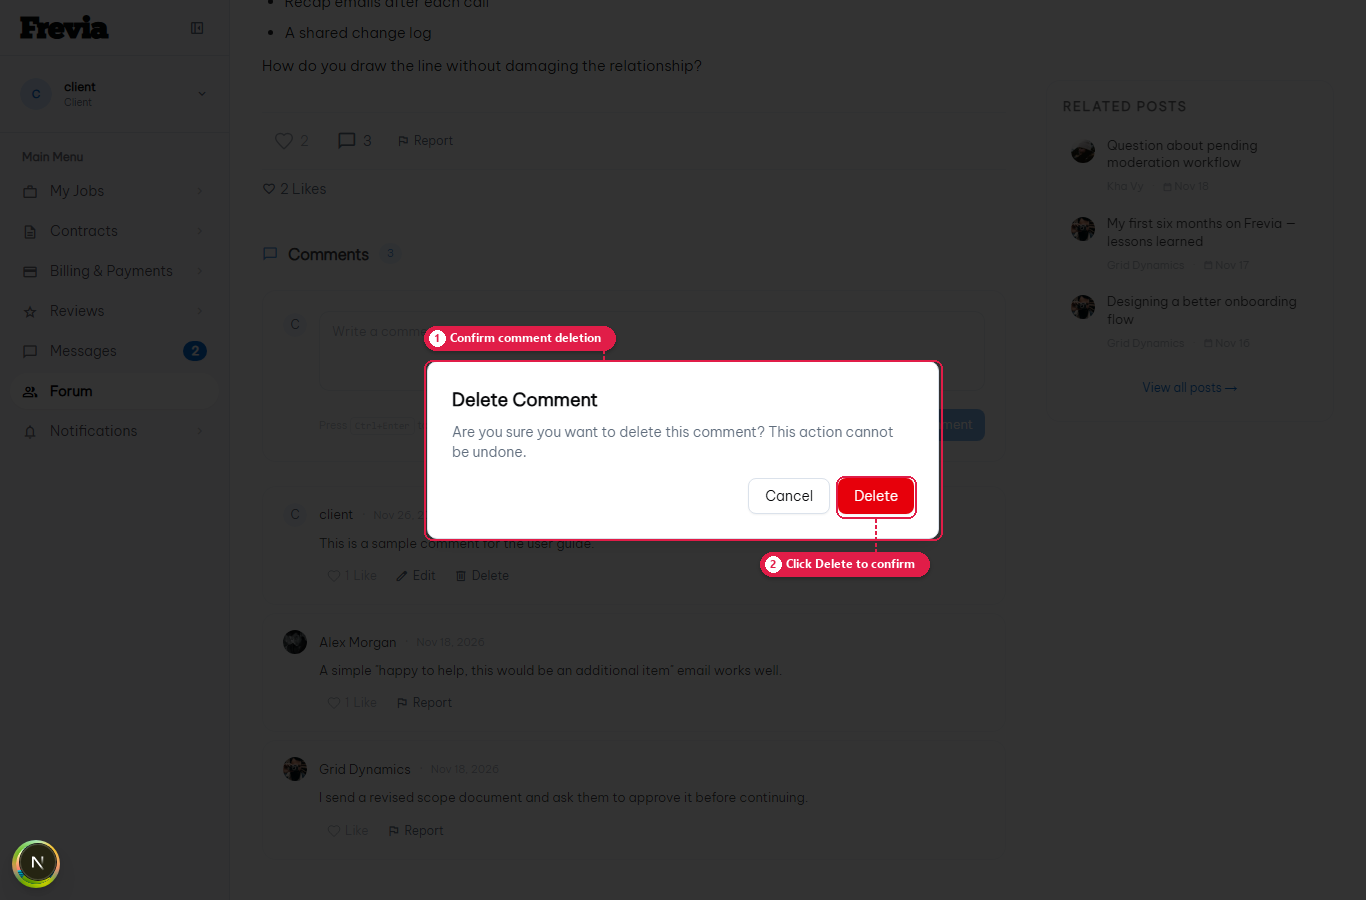
\includegraphics[width=0.90\textwidth]{images/forum/f14_14_guide.png}
  \caption{Soft-deleting a comment}
\end{figure}
\Needspace{6\baselineskip}\paragraph{Step-by-Step User Guide:}
\begin{enumerate}[leftmargin=1.8em,itemsep=3pt]
  \item \rbadge{1} \textbf{Click Delete:} Click \textbf{Delete} on your comment card.
  \item \rbadge{2} \textbf{Confirm Removal:} Confirm soft-deletion in the prompt modal.
\end{enumerate}
\Needspace{6\baselineskip}\paragraph{After You Submit (Result \& Troubleshooting):}
\begin{itemize}[leftmargin=1.5em,itemsep=2pt]
  \item \textbf{What Happens Next:} The comment is soft-deleted and hidden from public view.
  \item \textbf{Troubleshooting \& Common Messages:} Deleted comments remain recoverable by administrators in Forum Trash.
\end{itemize}

\subsubsection{M14.15 -- Like Comment (UC-14.15)}
\begin{itemize}[leftmargin=1.5em,itemsep=2pt]
  \item \textbf{Screen Name \& Route Path:} Comment Card -- \texttt{/forum/\{categorySlug\}/\{postSlug\}}.
  \item \textbf{Who Can Use This:} Client, Freelancer.
  \item \Needspace{6\baselineskip}\textbf{Before You Begin:} User is signed in.
\end{itemize}
\begin{figure}[H]\centering
  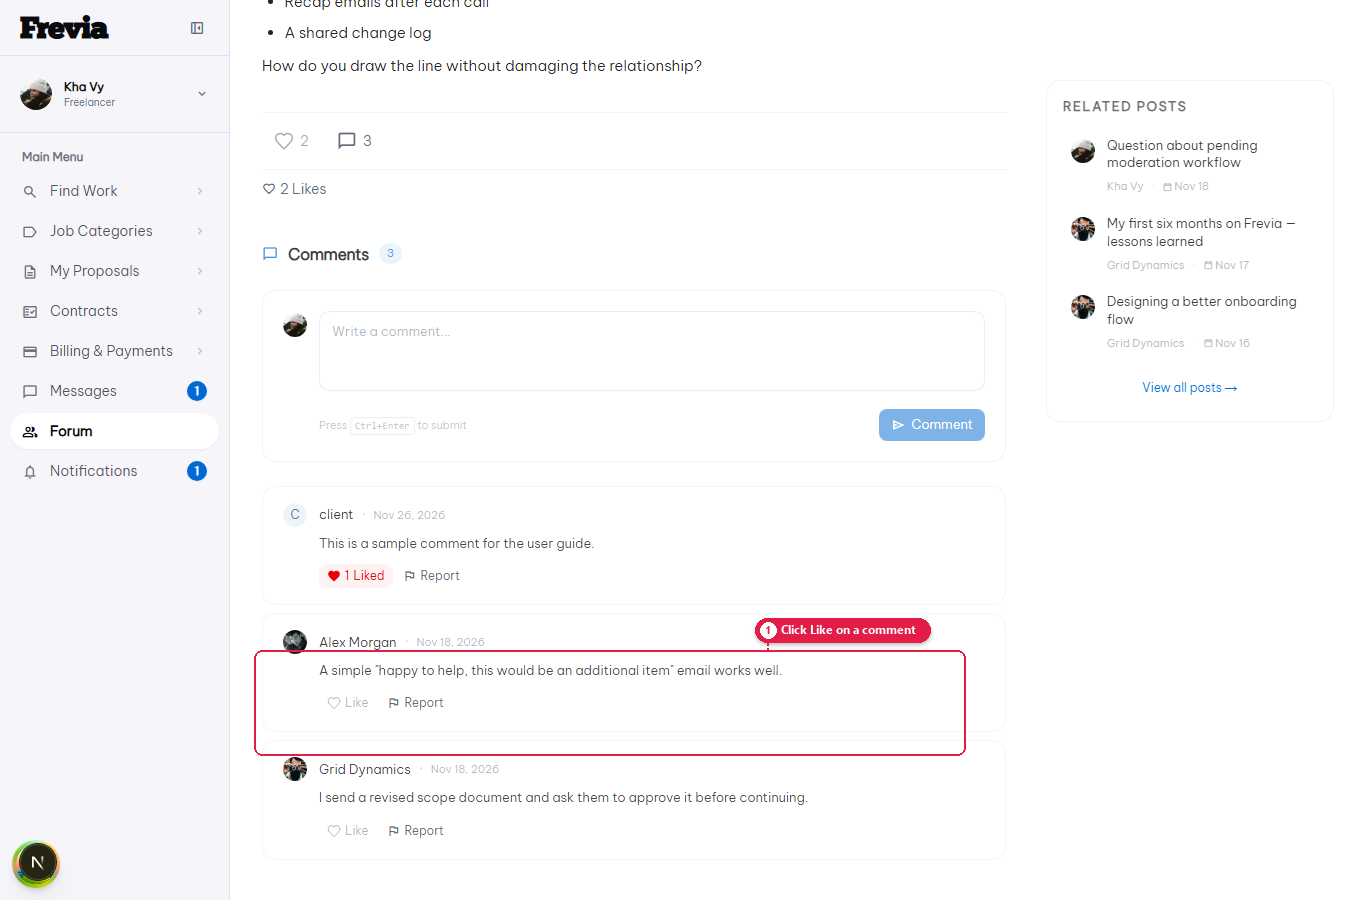
\includegraphics[width=0.90\textwidth]{images/forum/f14_15_guide.png}
  \caption{Liking a comment}
\end{figure}
\Needspace{6\baselineskip}\paragraph{Step-by-Step User Guide:}
\begin{enumerate}[leftmargin=1.8em,itemsep=3pt]
  \item \rbadge{1} \textbf{Click Like on Comment:} Click the Like icon on any helpful comment to upvote it.
\end{enumerate}
\Needspace{6\baselineskip}\paragraph{After You Submit (Result \& Troubleshooting):}
\begin{itemize}[leftmargin=1.5em,itemsep=2pt]
  \item \textbf{What Happens Next:} The comment like count increments immediately.
  \item \textbf{Troubleshooting \& Common Messages:} Duplicate likes by the same user are prevented.
\end{itemize}

\subsubsection{M14.16 -- Unlike Comment (UC-14.16)}
\begin{itemize}[leftmargin=1.5em,itemsep=2pt]
  \item \textbf{Screen Name \& Route Path:} Comment Card -- \texttt{/forum/\{categorySlug\}/\{postSlug\}}.
  \item \textbf{Who Can Use This:} Client, Freelancer.
  \item \Needspace{6\baselineskip}\textbf{Before You Begin:} User previously liked the comment.
\end{itemize}
\begin{figure}[H]\centering
  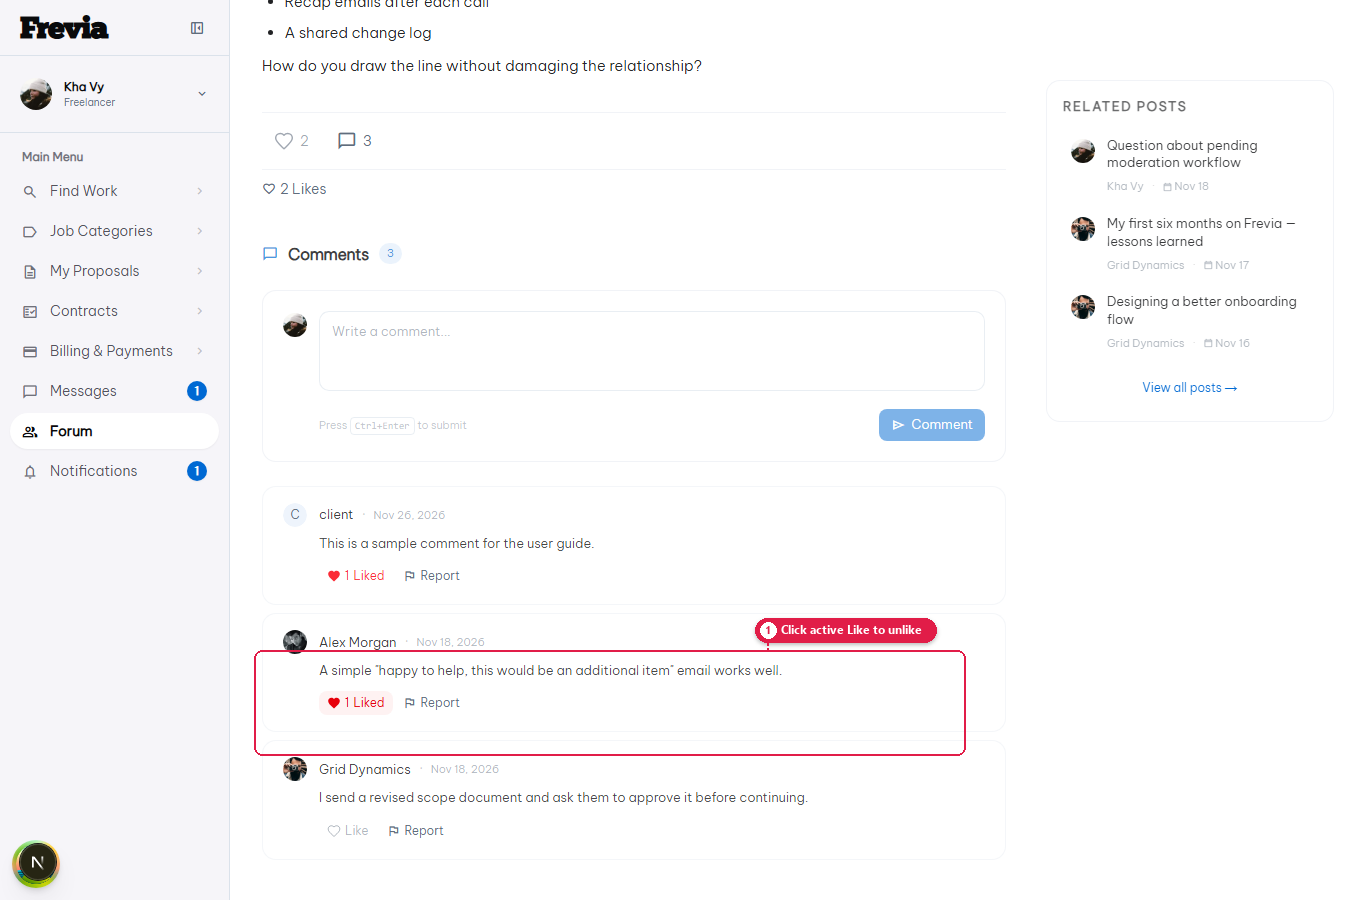
\includegraphics[width=0.90\textwidth]{images/forum/f14_16_guide.png}
  \caption{Unliking a comment}
\end{figure}
\Needspace{6\baselineskip}\paragraph{Step-by-Step User Guide:}
\begin{enumerate}[leftmargin=1.8em,itemsep=3pt]
  \item \rbadge{1} \textbf{Click Active Like:} Click the highlighted Like icon on the comment to remove your reaction.
\end{enumerate}
\Needspace{6\baselineskip}\paragraph{After You Submit (Result \& Troubleshooting):}
\begin{itemize}[leftmargin=1.5em,itemsep=2pt]
  \item \textbf{What Happens Next:} The comment like count decrements immediately.
  \item \textbf{Troubleshooting \& Common Messages:} If the comment was deleted, a warning toast is shown.
\end{itemize}

\subsubsection{M14.17 -- Report Content (UC-14.17)}
\begin{itemize}[leftmargin=1.5em,itemsep=2pt]
  \item \textbf{Screen Name \& Route Path:} Report Dialog -- \texttt{/forum/\{categorySlug\}/\{postSlug\}}.
  \item \textbf{Who Can Use This:} Client, Freelancer.
  \item \Needspace{6\baselineskip}\textbf{Before You Begin:} User is signed in and viewing a post or comment.
\end{itemize}
\begin{figure}[H]\centering
  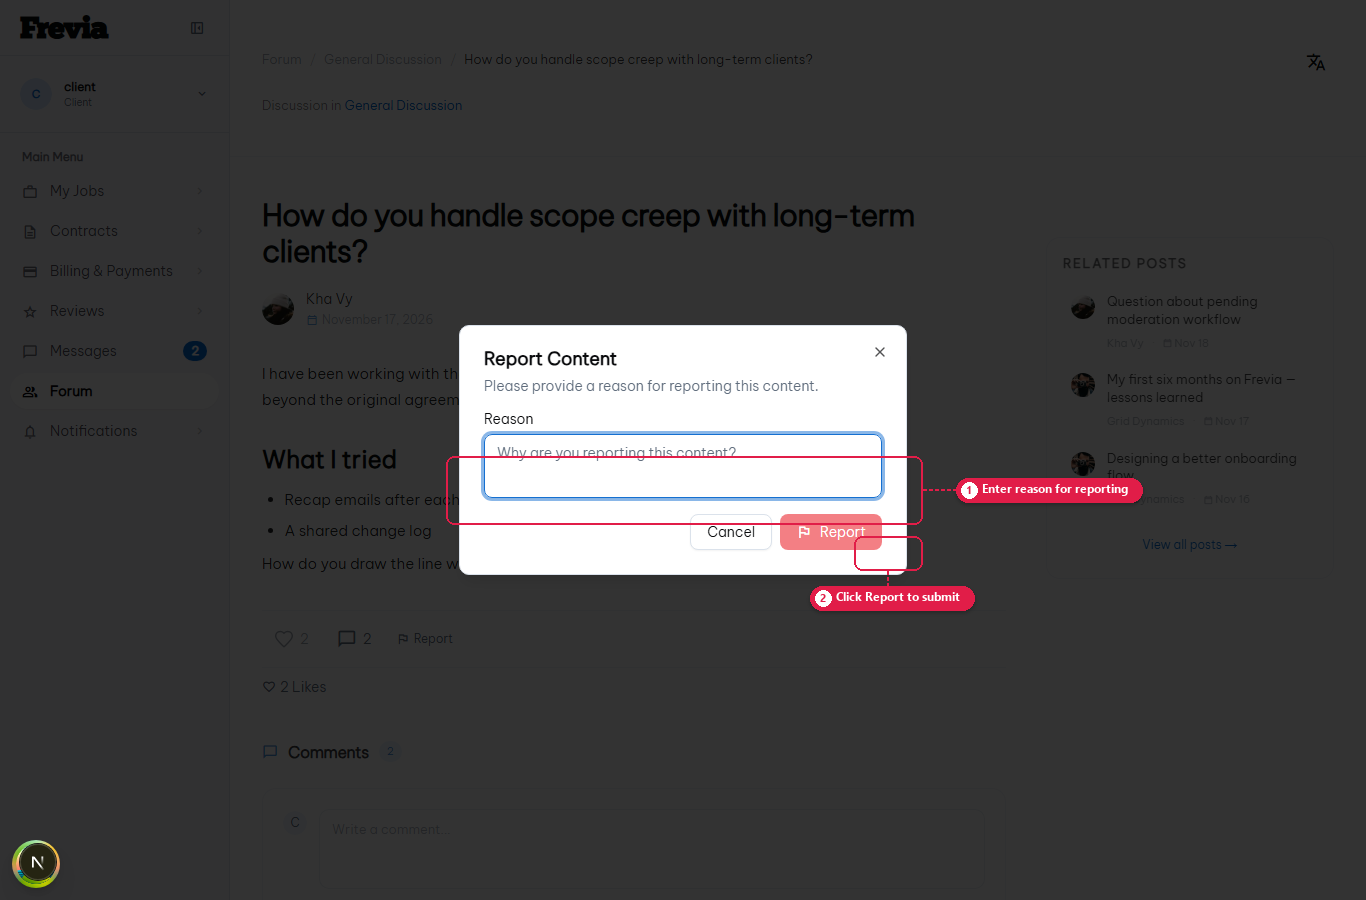
\includegraphics[width=0.90\textwidth]{images/forum/f14_17_guide.png}
  \caption{Reporting inappropriate forum content}
\end{figure}
\Needspace{6\baselineskip}\paragraph{Step-by-Step User Guide:}
\begin{enumerate}[leftmargin=1.8em,itemsep=3pt]
  \item \rbadge{1} \textbf{Click Report Flag:} Click the \textbf{Report} flag icon on the offending post or comment.
  \item \rbadge{2} \textbf{Select Reason \& Submit:} Choose a violation category, add optional context, and click \textbf{Submit Report}.
\end{enumerate}
\Needspace{6\baselineskip}\paragraph{After You Submit (Result \& Troubleshooting):}
\begin{itemize}[leftmargin=1.5em,itemsep=2pt]
  \item \textbf{What Happens Next:} A moderation report is created with status \texttt{PENDING} for administrator review.
  \item \textbf{Troubleshooting \& Common Messages:} Duplicate reports on the same item by the same user are blocked.
\end{itemize}

